\documentclass{article}
\usepackage[utf8]{inputenc}
\usepackage{hyperref}
\usepackage{geometry}
\usepackage{float}
\usepackage{graphicx}
\graphicspath{ {./figures/} }
\geometry{margin=1in}

\title{Rapport de Présentation de la Bibliothèque de Gestion des Digraphes et Circuits Booléens}
\author{Yehor KOROTENKO, Ivan KHARKOV, Sipan BAREYAN}
\date{\today}

\begin{document}

\maketitle

\section{Tâches Accomplies}
\begin{itemize}
    \item \textbf{Structure de Base du Graphe:}
    \begin{itemize}
        \item Implémentation de la classe \texttt{node} : Représente des nœuds individuels avec des identifiants uniques, des étiquettes et des relations parent/enfant.
        \item Développement de la classe \texttt{open\_digraph} : Gère les nœuds, les entrées/sorties désignées et fournit des méthodes pour ajouter/supprimer des arêtes et des nœuds.
    \end{itemize}
    \item \textbf{Opérations Avancées:}
    \begin{itemize}
        \item Ajout de la capacité de copie profonde, décalage des indices des nœuds et génération de correspondances d'identifiants séquentiels.
    \end{itemize}
    \item \textbf{Génération de Graphes Aléatoires:}
    \begin{itemize}
        \item Création de fonctions pour générer des matrices d'adjacence aléatoires (libres, symétriques, orientées, triangulaires) et conversion de ces matrices en digraphes via \texttt{open\_digraph.random()}.
    \end{itemize}
    \item \textbf{Extension aux Circuits Booléens:}
    \begin{itemize}
        \item Extension du graphe avec la classe \texttt{bool\_circ}, imposant des contraintes logiques telles que l'acyclicité et des degrés de nœuds appropriés.
    \end{itemize}
    \item \textbf{Visualisation:}
    \begin{itemize}
        \item Développement d'unu méthode de visualisation utilisant graphviz pour générer des graphiques en PDF, organisant les nœuds en sous-graphes d'entrée/sortie.
    \end{itemize}
    \item \textbf{Entrée/Sortie de Fichiers:}
    \begin{itemize}
        \item Implémentation de l'exportation vers des fichiers DOT et de l'importation depuis ces fichiers, permettant un stockage et une récupération persistants des données du graphe.
    \end{itemize}
    \item \textbf{La documentation}
    \begin{itemize}
        \item La documentation qui est stockée dans le répértoire \texttt{docs} qui décrit le fonctionnement des modules, méthodes, fonctions et provient les exemples d'utilisation.
    \end{itemize}
    \item \textbf{Collaboration et le répartition du travaille}
    \begin{itemize}
        \item Un dépot sur GitHub avait été crée dans lequel le code est souvegardé et partagé. Chaque membre de l'équipe a l'accès à ce dépot où chacun contribut du code.
    \end{itemize}
\end{itemize}

\section{Principales Fonctions et Descriptions}
\begin{itemize}
    \item \textbf{Fonctions de la Classe Node:}
    \begin{itemize}
        \item \texttt{get\_id()}, \texttt{get\_label()}, \texttt{set\_parents()}, etc.
        \item Gestion des arêtes : \texttt{add\_child\_id()}, \texttt{add\_parent\_id()}, \texttt{remove\_child\_once()}, \texttt{remove\_parent\_once()}.
        \item Calculs de degré : \texttt{indegree()}, \texttt{outdegree()}, \texttt{degree()}.
    \end{itemize}
    \item \textbf{Fonctions de \texttt{open\_digraph}:}
    \begin{itemize}
        \item Modifications du graphe : \texttt{add\_edge()}, \texttt{add\_node()}, \texttt{remove\_edge()}, \texttt{remove\_node\_by\_id()}.
        \item Gestion de l'état du graphe : \texttt{new\_id()}, \texttt{copy()}, \texttt{shift\_indices()}.
        \item Validation de la cohérence : \texttt{assert\_is\_well\_formed()}.
        \item Génération de matrices d'adjacence : \texttt{adjacancy\_matrix()}.
    \end{itemize}
    \item \textbf{Génération de Graphes Aléatoires:}
    \begin{itemize}
        \item Fonctions : \texttt{random\_int\_matrix()}, \texttt{random\_symmetric\_int\_matrix()}, \texttt{random\_oriented\_int\_matrix()}, \texttt{random\_triangular\_int\_matrix()}.
        \item Intégration via \texttt{open\_digraph.random()} permettant des paramètres tels que le nombre de nœuds, les bornes et les entrées/sorties désignées.
    \end{itemize}
    \item \textbf{Spécificités des Circuits Booléens (\texttt{bool\_circ}):}
    \begin{itemize}
        \item Hérite de \texttt{open\_digraph} et impose des contraintes logiques supplémentaires.
        \item Utilise \texttt{is\_well\_formed()} pour garantir l'acyclicité et la validité des degrés des nœuds.
    \end{itemize}
    \item \textbf{Module de Visualisation:}
    \begin{itemize}
        \item La méthode \texttt{display()} utilise Graphviz pour créer une représentation PDF du graphe.
    \end{itemize}
\end{itemize}

\section{Tests et Validation}
Tous les tests ont été exécutés avec succès à l'aide de la suite de tests fournie :
\begin{itemize}
    \item \textbf{Opérations sur les Nœuds et Graphes:} Test d'initialisation, ajout et suppression d'arêtes/nœuds, copie et calculs de degré.
    \item \textbf{Vérification de la Cohérence des Graphes:} Validation de la cohérence de \texttt{open\_digraph} et \texttt{bool\_circ} avec \texttt{assert\_is\_well\_formed()}.
    \item \textbf{Génération de Graphes Aléatoires:} Vérification que les fonctions génèrent les types de matrices corrects et des graphes conformes.
    \item \textbf{Entrée/Sortie des Fichiers DOT:} Test de l'exportation et de l'importation pour garantir la préservation des propriétés structurelles du graphe.
\end{itemize}
Les tests sont intégrés dans le framework \texttt{unittest} de Python et exécutés via le script shell \texttt{tests.sh}.

\section{Exemples d'Utilisation}
Voici quelques exemples démontrant les principales fonctionnalités de la bibliothèque :

\subsection*{Création d'un Graphe Aléatoire}
\begin{verbatim}
from modules.open_digraph import open_digraph

# Création d'un digraphe aléatoire avec 6 nœuds, une borne de 9, 1 entrée et 2 sorties
random_graph = open_digraph.random(n=6, bound=9, inputs=1, outputs=2)
\end{verbatim}

\subsection*{Création d'un Graphe concrète}
\begin{verbatim}
n0 = node(0, '0i', {3:1}, {1:1, 2:2})
n1 = node(1, '1i', {0:1}, {3:3})
n2 = node(2, '2o', {0:2}, {})
n3 = node(3, '3a', {1:3, 4:1}, {0:1})
n4 = node(4, '4i', {}, {3:1})
graph = open_digraph([4], [2], 
                  [n0, n1, n2, n3, n4])
\end{verbatim}

\subsection*{Sauvegarde dans un Fichier DOT}
\begin{verbatim}
# Sauvegarde du graphe généré dans un fichier DOT pour visualisation
graph.save_as_dot_file("./dot.dot")
\end{verbatim}

\begin{verbatim}
# Le résultat obtenu dans le fichier dot.dot
digraph G{
subgraph inputs{
rank=same;
v4 [label="4i" shape=diamond]
}
subgraph outputs{
rank=same;
v2 [label="2o" shape=box]
}
v0 [label="0i" ]
v1 [label="1i" ]
v3 [label="3a" ]
v0 -> v1;
v0 -> v2;
v0 -> v2;
v1 -> v3;
v1 -> v3;
v1 -> v3;
v3 -> v0;
v4 -> v3;
} 
\end{verbatim}

\subsection*{Importation et Affichage du Graphe}
\begin{verbatim}
from modules.open_digraph import open_digraph

# Importation du graphe depuis le fichier DOT
imported_graph = open_digraph.from_dot_file("./dot.dot")

# Affichage du graphe (Graphviz ouvrira un PDF)
imported_graph.display("imported_graph")
\end{verbatim}

\begin{figure}[H]
    \centering
    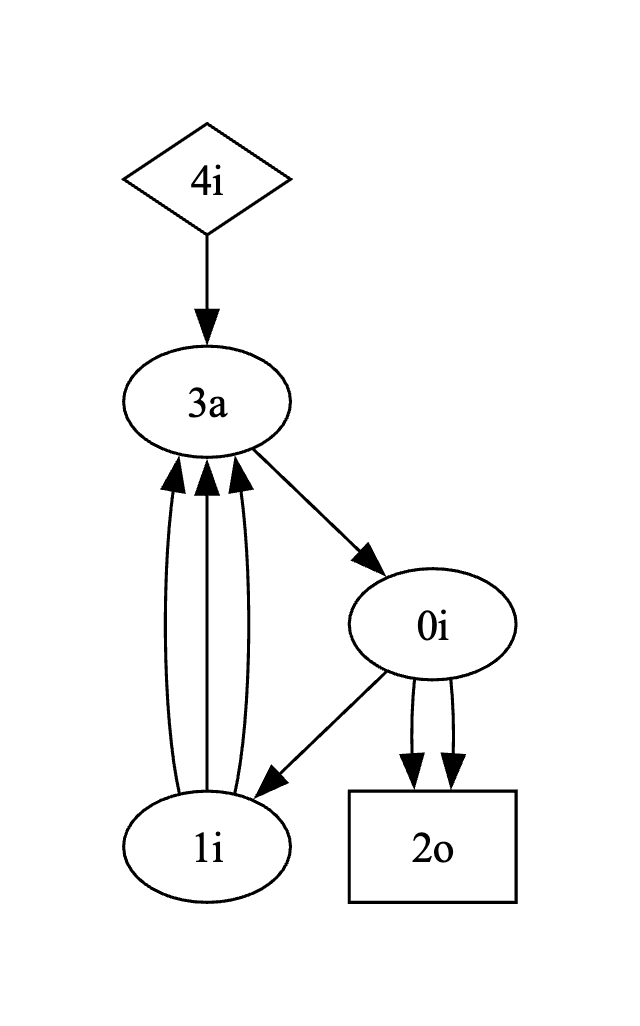
\includegraphics[width=0.8\textwidth]{graph.png}
    \caption{Affichage du graphe par \texttt{graph.display()}}
    \label{fig:}
\end{figure}

\end{document} 
